\documentclass[conference]{IEEEtran}
\IEEEoverridecommandlockouts
% The preceding line is only needed to identify funding in the first footnote. If that is unneeded, please comment it out.

\usepackage{amsmath,amssymb,amsfonts}
\usepackage{algorithmic}
\usepackage{textcomp}
\usepackage{xcolor}
\usepackage{nicefrac}  % nicer inline fractions
\usepackage{tensor}  % allows fancy indices
\usepackage{siunitx}  % easy handling of value + unit (e.g. \SI{10}{\pF})
% \sisetup{}  % configure siunitx (e.g. locale = DE)
\sisetup{output-complex-root=\ensuremath{\mathrm{j}}, complex-root-position = before-number} % configures SI format 10 + j5 for complex numbers (instead of 10 + 5i)

\usepackage{listings}
\usepackage{enumerate}
\usepackage{booktabs}  % nicer tables (e.g. \toprule)
\usepackage{verbatim}  % inline code (\verb||)
\usepackage[european, siunitx, RPvoltages]{circuitikz}  % draw circuit diagrams
\usepackage{enumitem}
\setlist[itemize]{label=\rule[0.5ex]{0.6ex}{0.6ex}} % black squares for itemize

\usepackage{graphicx}
\graphicspath{{./figures/}}

\usepackage{csquotes} % removes biber warning
\usepackage[  % ieee style citations (e.g. [1])
	backend     = biber,
	maxbibnames = 99,
	autocite    = footnote,
	style	    = ieee,
	citestyle   = numeric-comp,
	doi=false, isbn=false
]{biblatex}
\addbibresource{bibliography.bib}

\usepackage[nobiblatex]{xurl}  % line breaks in URLs
% last imports
\usepackage[bookmarksopen,colorlinks,citecolor=black,linkcolor=black, urlcolor = black]{hyperref}

% after hyperref! 
\usepackage[noabbrev, nameinlink]{cleveref} 
% e.g. \cref{label} or \Cref(label) for capital letter
% configure cleveref not to use brackets around equation references
\creflabelformat{equation}{#2\textup{#1}#3} % Equation references without parentheses
\AtBeginEnvironment{appendices}{\crefalias{section}{appendix}} % Appendix referencing (for cref "Appendix A" instead of "Section A")

\def\BibTeX{{\rm B\kern-.05em{\sc i\kern-.025em b}\kern-.08em
	T\kern-.1667em\lower.7ex\hbox{E}\kern-.125emX}}
	
	\lstdefinestyle{mystyle}{                
    captionpos=b,             
    tabsize=4
}

\lstset{style=mystyle}

\pagenumbering{arabic}

\begin{document}

\title{A Little Riscy: Implementation of a Simple Superscalar RISC-V Processor\\
{
\thanks{Submitted \today}
}
}

\date{\today}

\author{\IEEEauthorblockN{Severin Jäger}
severin.jaeger@tuwien.ac.at\\
Mat.Nr. 01613004\\

\and
\IEEEauthorblockN{Max Tamussino}
e1611815@student.tuwien.ac.at\\
Mat.Nr. 01611815\\
}

\maketitle

\begin{abstract}
\emph{A Little Riscy} is a minimalistic superscalar RISC-V processor featuring parallel execution of ALU and load/store instructions. Due to its four-stage pipeline it is able to efficiently handle data hazards, however its performance decreases drastically when branching is involved. Thus, it shows that superscalar processors do not only need parallel execution units, but also compiler support and branch prediction with speculative execution to achieve a high IPC outside artificial mixes of instructions.
\end{abstract}

\section{Introduction}
The open RISC-V instruction set architecture \cite{risc-v} has gained significant popularity both in academia and in industry. Within the \emph{Advanced Computer Architecture} course at TU Wien, a minimalistic superscalar RISC-V processor called \emph{A Little Riscy} has been designed. It implements the RV32I instruction set and allows parallel execution of ALU and load/store instructions with in-order dual issue.

Due to the limited scope of this project, several instruction level parallelism techniques were not implemented. These include branch prediction and speculative execution as well as out-of-order issuing.

This report covers the implemented architecture of the processor in Section~\ref{sec:implementation}, some evaluation results in Section~\ref{sec:eval} and a discussion of the design including potential improvements in Section~\ref{sec:conclusion}.

\begin{figure}[h]
	\centering
	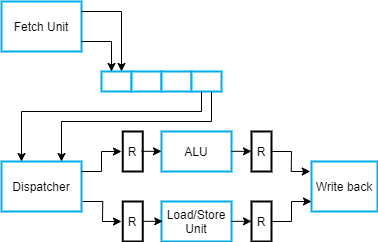
\includegraphics[width=7cm]{basic_architecture_2.PNG}
	\caption{Basic structure of the implemented processor \cite{Hamacher}}
	\label{fig:basic_arch}
\end{figure}

\section{Implementation} \label{sec:implementation}
The implemented processor follows the architecture depicted in Figure~\ref{fig:basic_arch}. Thus, it features a Harvard architecture with a four stage pipeline (Fetch, Dispatch, Execute, Write Back) with an ALU and a load/store unit in parallel in the execution stage. In order to utilise the parallel execution units, two instructions per cycle are fetched, enqueued, dequeued and dispatched respectively. The whole design was implemented using the Chisel hardware description language.

As the evaluation of the processor was conducted with rather simple single-threaded programs (cf. Section~\ref{sec:eval}), the following instructions were not implemented and are thus interpreted as NOP: FENCE, ECALL, EBREAK. Otherwise, \emph{A Little Riscy} is except for some memory limitations (cf. Section~\ref{sec:memory}) compliant with the RV32I instruction set.

\subsection{Fetch Unit} \label{sec:fetch}
The fetch unit loads two instructions per cycle from the instruction memory and places them into the instruction queue. Additionally, it administrates the PC. In case the queue is full, the whole fetching process is stalled.

Furthermore, it implements all control flow transfer instructions. This implies the following:
\begin{itemize}
	\item As there is no ALU in a previous pipeline stage, additional hardware is required for address calculations.
	\item To ensure the correct register values are present while calculating addresses, the fetch unit has to wait for all previous instructions to take effect before the calculation. This implies that no instructions can be queued until the whole pipeline is idle.
\end{itemize}

The latter can in principle be mitigated using branch prediction and speculative execution techniques, however this was outside the scope of this project.

In case a jump or branch instruction is dequeued, the fetch unit performs the following steps.
\begin{itemize}
	\item Stall the pipeline (by scheduling NOPs)\footnote{The instruction loaded from the instruction memory is still dispatched in case its PC is lower than the one of the branch instruction.}.
	\item Wait for the dispatcher to report an empty pipeline (i.e. all register values are written).
	\item Decode the branch instruction, calculate the target and determine whether the branch is taken.
	\item Enqueue an ADDI instruction writing the address of the instruction after the jump (only applicable for jumps).
	\item Continue with regular fetch operation.
\end{itemize}

\subsection{Instruction Queue}
The instruction queue is a simple register based FIFO (cf. the \verb|RegFifo| in \cite{schoeberl}) with a width of $96$~bits ($2\times32$~bits instruction, $32$~bits PC) and a depth of $4$. This brings the limitation that only the two instructions being enqueued together can be dequeued at the same time. In case of structural hazards (i.e. only one of the loaded instructions can be issued), this leads to a serialised processing.

\subsection{Dispatcher} \label{sec:dispatch}

\begin{figure}
	\centering
	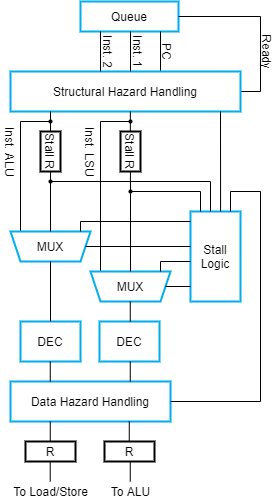
\includegraphics[width=5cm]{dispatcher.png}
	\caption{High-level schematic of the implemented dispatcher}
	\label{fig:dispatcher}
\end{figure}

The dispatcher dequeues two instructions and issues them to the execution units (ALU and load/store). It is of utmost importance, that structural and data hazards are resolved beforehand. This is done by the means of operand forwarding and stalling of conflicting instructions.

The treatment of structural hazards is done as the following: In case two instructions for the same execution unit or with identical destination register are dequeued, the first one is issued while the second is stalled in special stall registers (s. Figure~\ref{fig:dispatcher}). In the next cycle, no new instructions are dequeued and the stalled instruction is issued.

Afterwards, the instructions are decoded (in parallel for ALU and load/store), then data hazards can be treated. This is done by comparing the operand register addresses with the destination register of instructions in the current and the last cycle. In case there is a data hazard related to an instruction dispatched in the last cycle, operand forwarding can be used to resolve this issue without stalling the pipeline\footnote{This is not the case for the standard five stage RISC pipeline proposed in~\cite{HP}.} So in this case, the dispatcher only has to calculate the forwarding signals shown in Figure~\ref{fig:dispatcher}.

However, in case instructions decoded during the same cycle impose some ordering constraints, the instruction with the higher PC has to be stalled. This is done in the same fashion as the instruction stalling for structural hazards and delays instructions for one cycle.

In principle, all aforementioned hazards can be resolved by implementing an dynamic scheduling approach like Tomasulo´s algorithm. However, this is not suitable for the chosen architecture. This is due to the common data bus, which broadcasts the results of all calculations to the reservation stations and the register bank. This bus need some arbitration policy to prevent two execution units from broadcasting their results simultaneously. However, in the case of \emph{A Little Riscy} both execution units generate one result per cycle respectively\footnote{This is not the case for floating point units, where individual instructions usually take multiple cycles.}. Thus, the bandwidth of the basic single-word bus is not sufficient. This leads to a major bottleneck for the whole pipeline.

\subsection{Arithmetic Logic Unit}
This execution unit implements all instructions listed in Section~$2.4$ of the RISC-V Specification~\cite{risc-v}. The LUI and the AUIPC instruction as well as the operand forwarding described in Section~\ref{sec:dispatch} require a dynamic allocation of the operands. This is achieved by the means of multiplexers with select signals created by the dispatcher. This is depicted in Figure~\ref{fig:alu}.

\begin{figure}
	\centering
	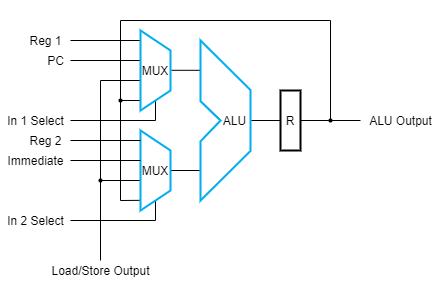
\includegraphics[width=7cm]{alu_mux.png}
	\caption{ALU with input multiplexers for operand forwarding}
	\label{fig:alu}
\end{figure}

\subsection{Load/Store Unit} \label{sec:load_store}
The load/store unit handles all accesses to the data memory. It implements all respective instructions in the RV32I instruction set, the only limitations are discussed in the next section. Similar to the ALU, its inputs feature multiplexers to allow for the use of forwarded values.

\subsection{Registers} \label{sec:registers}
The register bank consists in compliance with the RISC-V reference manual out of 32 general purpose registers (x0 is always set to zero) and the program counter. The architecture demands six read ports (two for the ALU, two for the load/store unit and two for the fetch unit) and two write ports (one for ALU and load/store unit respectively).

\subsection{Memory System} \label{sec:memory}
As \emph{A Little Riscy} implements a Harvard architecture, instruction and data memory are separated. The instruction memory is a read-only type, holds $128$ word (and thus instructions), and is only word addressable. Due to their small size, both can be implemented as registers. In contrast the $256$ word data memory allows byte, halfword and word addressing, however it assumes aligned halfwords and words both for reads and writes.

\subsection{Performance Considerations} \label{sec:performance}
From the previous sections, the following statements about the theoretically achievable performance can be made:
\begin{itemize}
	\item As the data memory is implemented as register, there is no memory delay, so load/store instructions take as long as ALU instructions.
	\item In the absence of pipelining hazards, two instructions per cycle can be executed, thus a IPC of $2$ is the upper bound for this processor.
	\item Instructions with data hazards can be executed without any additional delay as long as they are not fetched simultaneously.
	\item Branching requires completion of all previous instructions and thus introduces significant idle time.
	\item The instruction queue adds latency to the pipeline, this is unfavourable in the beginning and during branches.
\end{itemize}

Thus, efficient code for \emph{A Little Riscy} consist of interleaved load/store and ALU instructions and minimises the number of control flow transfer instructions. The following section investigates these observations empirically.

\section{Evaluation} \label{sec:eval}

\subsection{Benchmarks}

In order to evaluate the performance of the implemented processor some benchmarks were conducted. Thereto short C programs were compiled using the \href{https://github.com/riscv/riscv-gnu-toolchain}{RISC-V GNU Compiler Toolchain}. All experiments were conducted in a Chisel Tester based simulation environment.
 
The first benchmark aims at evaluating the performance of the processor with specialised ALU load. Listing~\ref{code:alu} shows the respective C code which was compiled with the \verb|-O3| flag. Afterwards, the instructions loading the value of the global variables used as input\footnote{This is done in order to exploit the compilers optimiser without losing the actual implementation.} from memory were replaced by simpler load immediate instructions.

\begin{lstlisting}[language=C, caption=Code for the ALU benchmark, label=code:alu]
	int A = 13;
	int B = 2;
	int C = 11;
	int D = 7;

	int main() {
		int a = A;
		int b = B;
		int c = C;
		int d = D;
		int r =  ((((a+5-b) << 3) >> b) -
				((c | a) - 9)) ^ (d+2);
	}
\end{lstlisting}

The code for the second benchmark is depicted in Listing~\ref{code:loop}. It consist of two loops, one setting the elements of an array to \verb|i+1| and the second one is summing up its elements. This is compiled with the \verb|-O1| flag. The resulting assembly code contains numerous branch instructions due to the implemented loops. Thus, frequent control flow transfers occur.

\begin{figure}
	\centering
	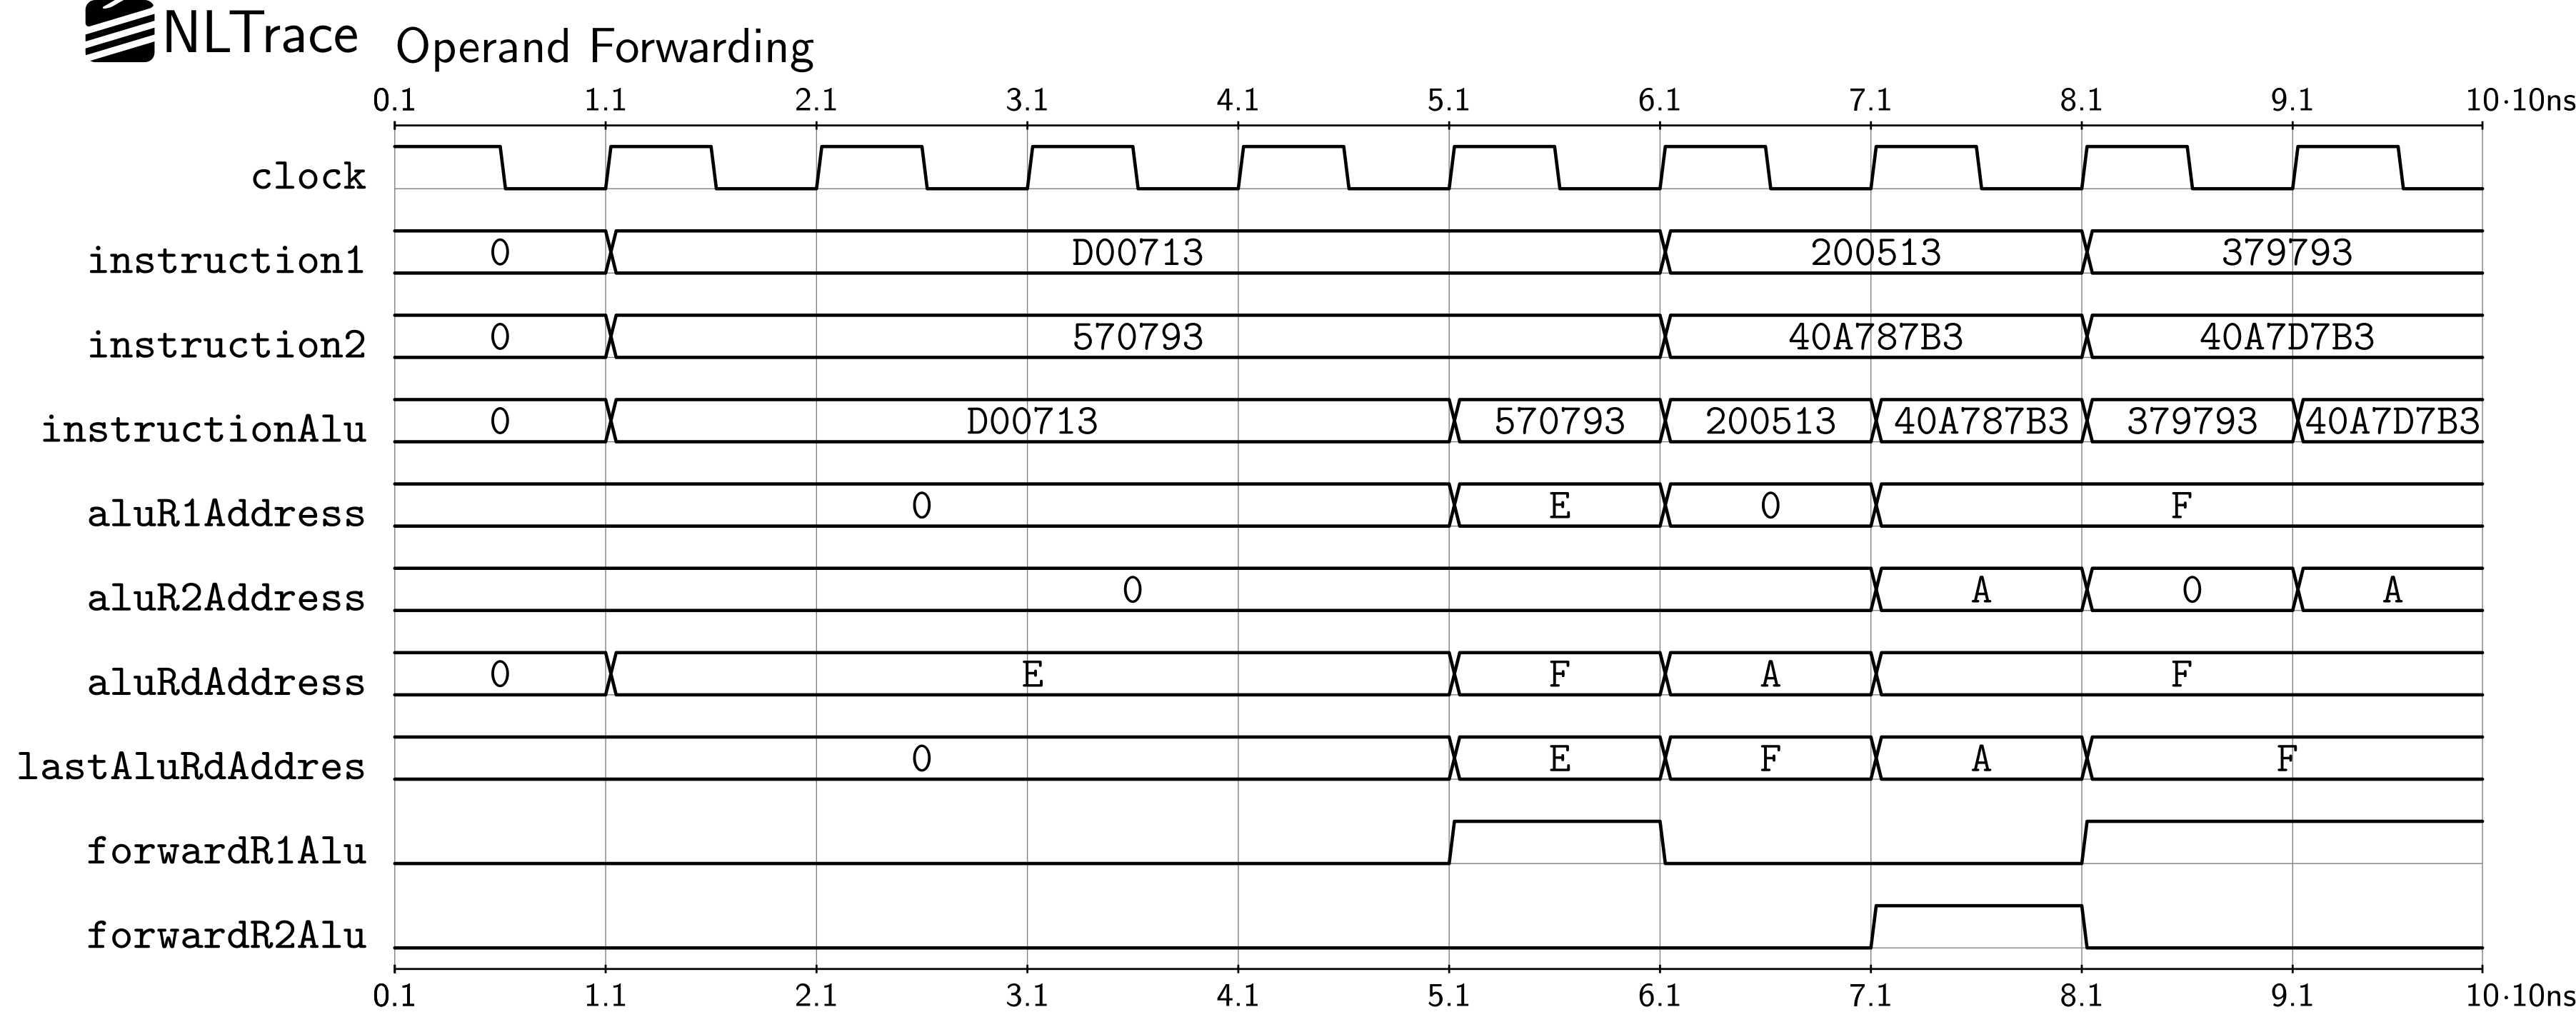
\includegraphics[width=8.7cm]{vcd_forwarding.png}
	\caption{Dispatcher signals for operand forwarding in the ALU benchmark}
	\label{fig:vcd_alu}
\end{figure}


\begin{lstlisting}[language=C, caption=Code for the loop benchmark, label=code:loop]
	int N = 5;
	int main() {
		int n = N;
		int a[5] = {};

		int i = 0;
		for(;i<n;i++) {
			a[i] = i+1;
		}
		int r = 0;
		for(i=0;i<n;i++) {
			r += a[i];
		}
		return r;
	}
\end{lstlisting}

The third benchmark uses the code from Listing~\ref{code:loop} again, however it was compiled with the \verb|-O3| flag, which resulted in an unrolled loop. Some minor rearrangements have been made in order to ensure efficient utilisation by interleaving of ALU and load/store instructions.

\begin{figure*}
	\centering
	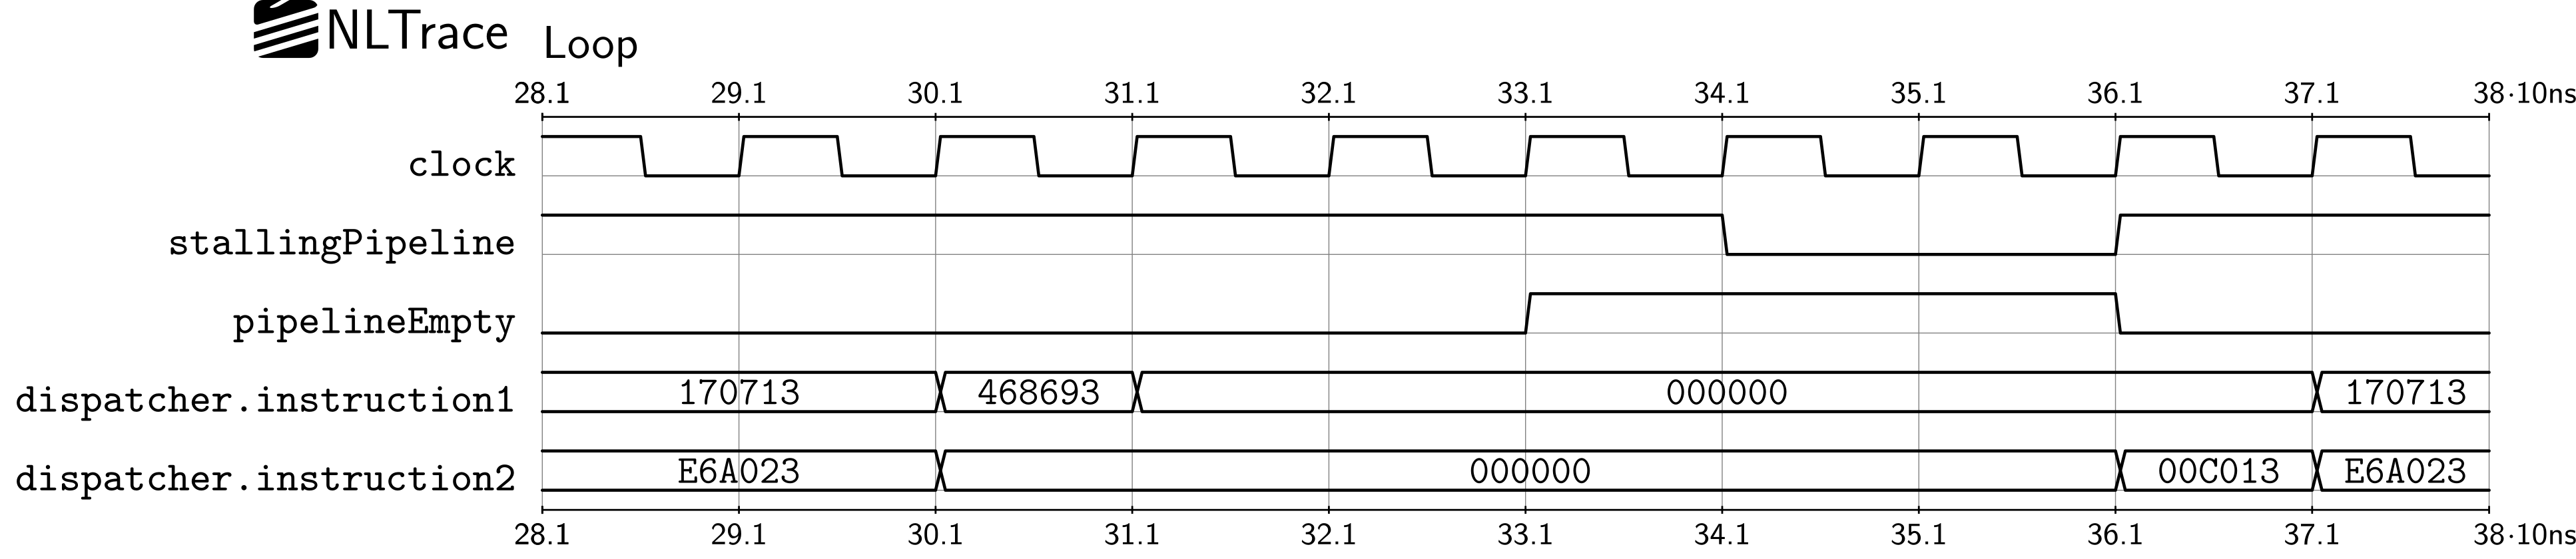
\includegraphics[width=0.65\textwidth]{vcd_loop.png}
	\caption{Dispatcher signals in the loop benchmark. No instructions are scheduled during branches, this leads to significant idle time.}
	\label{fig:vcd_loop}
\end{figure*}


The benchmarking results are summed up in Table~\ref{tab:results}. Note that the latency of the pipeline is subtracted from the measured number of cycles in order to measure independent of the length of the code. Thus, the maximum theoretically achievable IPC is $2$.

\begin{table} [h]
	\caption{Benchmarking results}
	\centering
	\begin{tabular}{l c c c}
			Benchmark & Instructions & Cycles & IPC \\
		\midrule
			ALU & 13 & 13 & 1 \\
			Loop & 52 & 108 & 0.48 \\
			Loop Unrolled & 27 & 21 & 1.29
	\end{tabular}
	\label{tab:results}
\end{table}


The ALU benchmark, which consists only of ALU instructions, leads to an IPC of $1$. Note that the ALU instructions have to be serialised because there is only one ALU available, the load/store unit is idle during the whole benchmark. Thus, more instructions per cycle are not achievable. This maximum could be reached due to the implementation of operand forwarding. This technique enables handling of the occurring data hazards without introducing any delay. This is shown exemplarily in Figure~\ref{fig:vcd_alu}.

The simple loop benchmark shows the weak spots of the processor. The IPC drops significantly below $1$, this is mainly due to the negative effects of branching (cf. Section~\ref{sec:fetch}). The waveforms in Figure~\ref{fig:vcd_loop} shows one iteration of the first loop and indicates that branch instructions force the pipeline to be idle for significant timespans.

The unrolled loop is able to cope with this problem. As branch instructions were removed, the performance is limited by the distribution between ALU and load/store unit instructions. As long as one load/store and one ALU instruction is issued per cycle, the IPC is $2$, it only drops within phases of sequential ALU or load/store instructions or when destination register conflicts occur. This is shown in Figure~\ref{fig:vcd_loop_unrolled}.

\begin{figure}
	\centering
	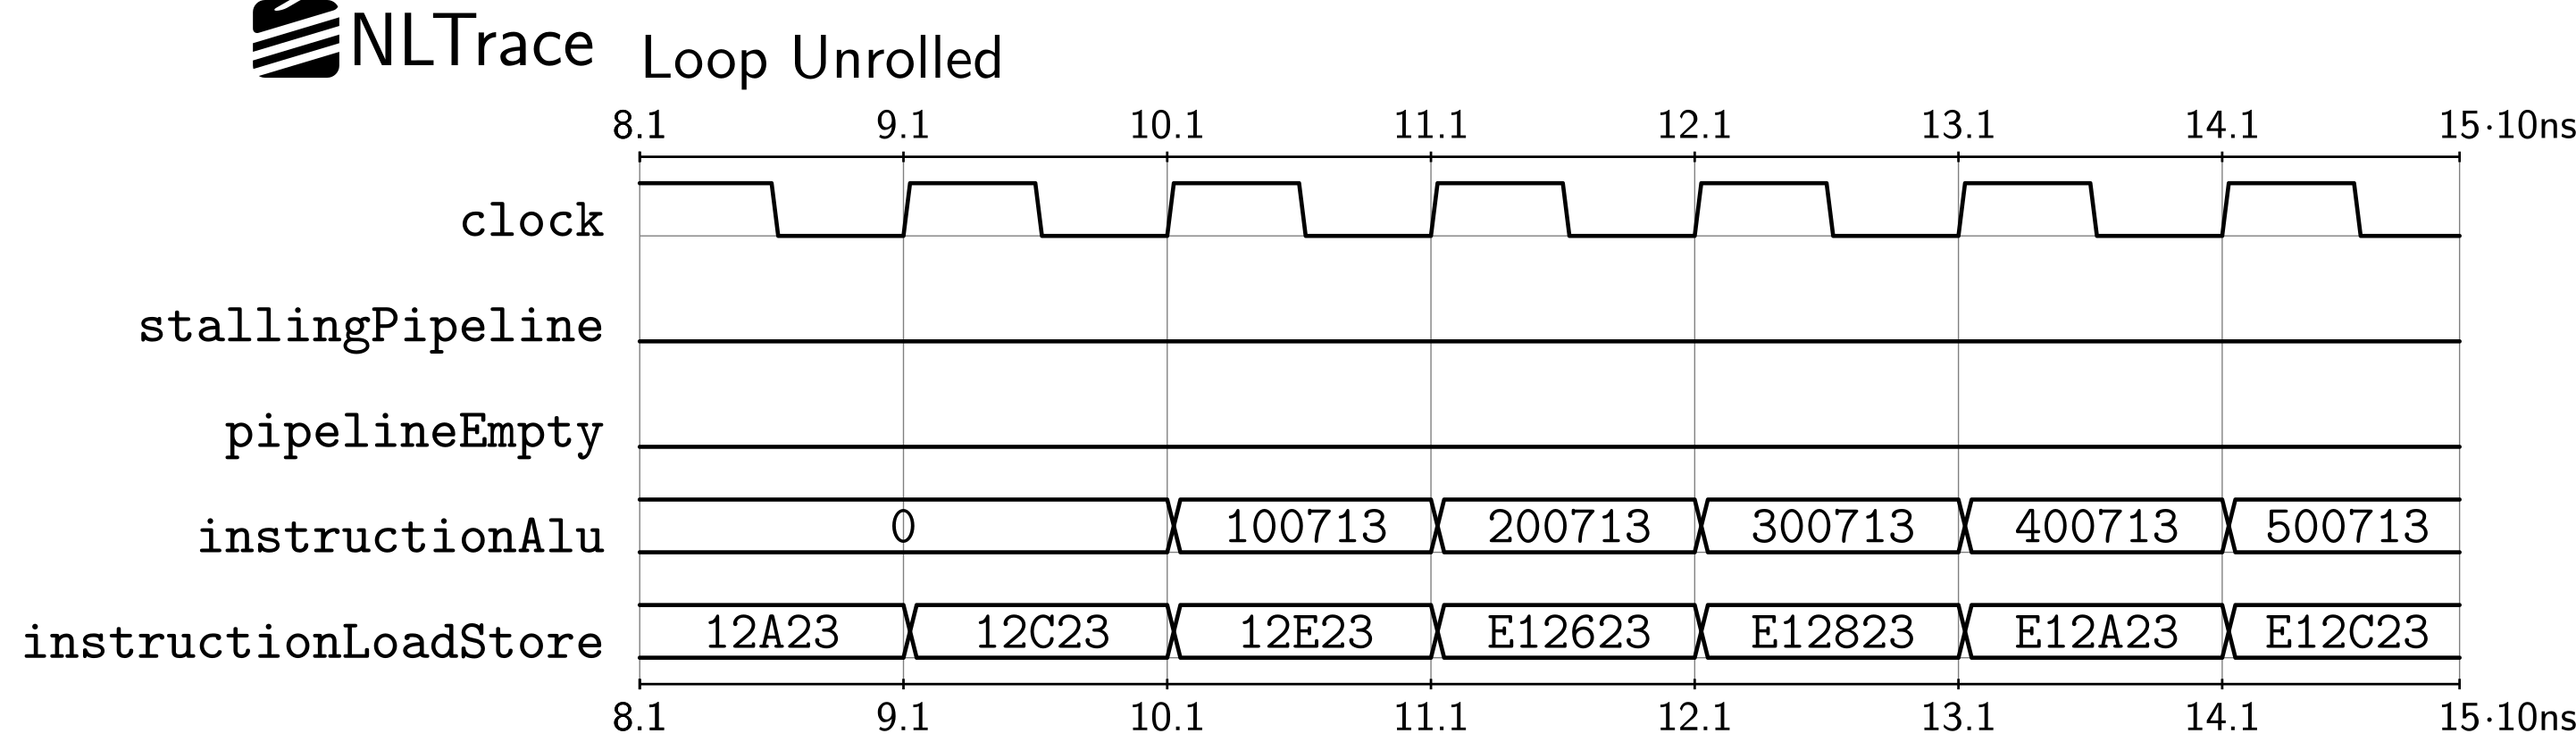
\includegraphics[width=8.7cm]{vcd_loop_unrolled.png}
	\caption{Dispatcher signals in the unrolled loop benchmark. The first two instructions are both load/store instructions, they are therefore executed sequentially. Afterwards, ALU and load/store instructions are interleaved, the design is exploited efficiently.}
	\label{fig:vcd_loop_unrolled}
\end{figure}


\subsection{FPGA Evaluation}

\begin{table}
	\caption{Resource consumption of the different units on the target FPGA}
	\centering
	\begin{tabular}{l c c c}
			Entity & LUTs & Registers & Logic Cells \\
		\midrule
			ALU & 1929 & 38 & 1967 \\
			Dispatcher & 357 & 191 & 548 \\
			Fetch Unit & 501 & 55 & 556 \\
			Instruction Memory & 121 & 0 & 121 \\
			Load/Store Unit & 864 & 69 & 933 \\
			Data Memory & 2431 & 8192 & 10623 \\
			Instruction Queue & 12 & 342 & 354 \\
			Register & 1125 & 1024 & 2149 \\
		\midrule
			Total & 7340 & 9825 & 17165 \\
	\end{tabular}
	\label{tab:resources}
\end{table}

An Altera DE2-115 evaluation board featuring an Altera Cyclone IV FPGA was used as hardware platform. The resource usage of the implemented processor is shown in Table~\ref{tab:resources}. 
The notably high number of logic required for the register bank is due to the high number of read and write ports (cf. Section~\ref{sec:registers}).

The maximum available clock frequency for this design is \SI{29.1}{\MHz}. The critical path runs through the dispatcher (between input and output of the stall registers, s. Figure~\ref{fig:dispatcher}). This is hardly surprising as the dispatcher has a rather complex task. Finer pipelining i.e. splitting the dispatcher into two stages might be a solution to increase the clock frequency.

\section{Conclusion and Outlook} \label{sec:conclusion}

During this project, a simple superscalar RISC-V processor with one ALU and one load/store unit in parallel was implemented. It is capable of executing up to two instructions per cycle, however benchmarks have showed that this requires a rather artificial mix of instructions. Especially branching causes significant performance drops as neither branch prediction nor speculative execution were implemented.

In general, it can be concluded that instruction level parallelism is an interesting way to increase the performance of a processor, however there are two requirements that have to be satisfied in order to reach an IPC significantly above $1$:

\begin{itemize}
	\item The compiler has to optimise with the architecture in mind and make sure that instructions are ordered in a suitable way for superscalar machines. This mainly involves suitable loop unrolling and interleaving of different instruction types.
	\item Going superscalar does not only require parallel execution units, but an all-in approach covering several modern ILP techniques (like the ones presented in.~\cite{HP}). This includes branch prediction and speculative execution in order to reduce the branch penalty as well as out-of-order issuing. However, the come at the cost of additional transistors as well as significantly increased design complexity.
\end{itemize}


\printbibliography

\end{document}